%\linenumbers*
\chapter{IMPLICATION OF IMPROVED CLIGEN ON RAINFALL AND SOIL EROSION
SIMULATIONS}
\label{sec:IMPLICATIONSOFIMPROVEDCLIGEN}

\section{Introduction}
\label{sec:ImprovedCligenIntroduction}
CLIGEN, a weather generator for WEPP, went through extensive modifications while
the current research was carried out \citep{yu2000-301}. The modification was
done to improve CLIGEN in three aspects. The first is the recalculation of an
input parameter, `{MX.5P}', which controls rainfall intensity generations of
CLIGEN. The second is the correction of the unit conversion error in programming
codes of CLIGEN. The third is a subsequent adjustment to shorten the extensive
increases of simulated rainfall durations.

These unforeseen changes prompted an investigation of their implications on
rainfall generations of CLIGEN and, in turn, soil erosion estimations of WEPP.
Before using the improved CLIGEN, it is important to understand how the improved
CLIGEN perform and simulates weather data in comparison to the previous version.
Also, how these changes of CLIGEN affect on previous publications needs to be
discussed.

Therefore, this chapter investigates effects of the changes of CLIGEN (from
version 4.2 to version 5.2) on rainfall data simulations and soil erosion
estimations by WEPP. During the investigation process, WEPP is also calibrated
and used for the subsequent simulations of this thesis. Some previous
publications have been identified later in this chapter in regard to
implications of CLIGEN changes.

\section{Data Preparation and Method for Model Simulation}
\label{sec:ImprovedCligenMethods}
Firstly, two CLIGEN input files---original and updated (see Appendix
\ref{sec:CLIGENInputData})---were prepared using more recent rainfall data
(Table \ref{tab:DetailsOfDataStations}) obtained from the Ditchling Road site
(Figure \ref{fig:EventRainfallDataSite}). The original CLIGEN input file for
Ditchling Road was used in a study by \citet{favis-mortlock1998-141}. This file
was originally built with help from Arlin Nicks for David Favis-Mortlock in
1992\footnote{From personal communication with David Favis-Mortlock on 3 July
2001: \begin{quotation} ``My problem was that, in 1992, I did not have any
measured intensity data for the area. So, as I recall, I used maps in `NERC
(1975) \textit{Flood Studies Report}, Natural Environment Research Council,
HMSO, London' to pick out the maximum $x$-hour precipitation for each month for
the South Downs, where $x$ is something like 6 hours. The 1975 NERC report was
based on approximately 30 years of data. I then used a chart constructed from
empirical relationships in the 1975 NERC publication---Actually, from data given
to me by someone in the old Southern Water company, which data was drawn from
the 1975 NERC publication---to convert these values into 0.5-hour maxima. I then
sent these 0.5-hour max.\ values to Arlin. From these he calculated time-to-peak
values.'' \end{quotation}}. The newly prepared CLIGEN input file used event data
that have been measured since 1991 (Table \ref{tab:DetailsOfDataStations}).
`MEAN~P' (Table \ref{tab:UpdatedMEANPForDitchlingRoad}) and `{MX.5P}' (Table
\ref{tab:UpdatedMX5PForDitchlingRoad}) values of CLIGEN inputs were recalculated
using the up-to-date event data. Note that the units for these parameters are in
inches, not in millimetres. Only these two parameters were updated because
rainfall intensity is closely related to these two parameters. The definition of
the `{MX.5P}' was revised by \citet{yu2000-301}, so it was recalculated
accordingly in this research.

\begin{table}[htbp]
  \centering
  \small
  \caption{Weather simulation settings with different CLIGEN versions and inputs
for Ditchling Road}
  \label{tab:CLIGENSimulationSettingsWithDifferentInputsAndVersions}
  \begin{tabular}{ccc}
  \toprule
        & Original Input & Updated Input \\
  \midrule
  CLIGEN v4.1 & v4.1+original & v4.1+updated \\
  \midrule
  CLIGEN v5.2 & v5.2+original & v5.2+updated \\
  \bottomrule
  \end{tabular}
\end{table}

Next, continuous daily climate data for 30 years were generated with CLIGEN
version 4.1\footnote{There is virtually no difference between version 4.1 and
4.2 although version 4.2 was the one \citet{yu2000-301} found error in.} (old)
and version 5.2 (new) using these two input files. As a result, four datasets of
simulated climate data were generated (Table
\ref{tab:CLIGENSimulationSettingsWithDifferentInputsAndVersions}). These climate
data were compared in terms of rainfall amount, duration and peak intensity.

\begin{table}[htbp]
  \figureversion{tabular}
  \centering
  \caption[Original and Updated MEAN~P for Ditchling Road]{Original and
Updated MEAN~P (inches) for Ditchling Road}
  \label{tab:UpdatedMEANPForDitchlingRoad}
    \footnotesize
    \begin{tabular}{lrrrrrrrrrrrr}
    \toprule
     & Jan & Feb & Mar & Apr & May & Jun & Jul & Aug & Sep & Oct &
Nov & Dec\\
    \cmidrule{2-13}
    Original & 0.19 & 0.16 & 0.17 & 0.16 & 0.16 & 0.20 & 0.19 & 0.22
& 0.23 & 0.27 & 0.21 & 0.20\\
    Updated & 0.11 & 0.11 & 0.18 & 0.21 & 0.17 & 0.15 & 0.16 & 0.13
& 0.24 & 0.29 & 0.19 & 0.29\\
    \bottomrule
    \end{tabular}
\end{table}

\begin{table}[htbp]
  \figureversion{tabular}
  \centering
  \caption[Original and Updated {MX.5P} for Ditchling Road]{Original and
Updated {MX.5P} (in/hr) for Ditchling Road}
  \label{tab:UpdatedMX5PForDitchlingRoad}
    \footnotesize
    \begin{tabular}{lrrrrrrrrrrrr}
    \toprule
     & Jan & Feb & Mar & Apr & May & Jun & Jul & Aug & Sep & Oct &
Nov & Dec\\
    \cmidrule{2-13}
    Original & 0.63 & 0.59 & 0.55 & 0.55 & 0.55 & 0.55 & 0.55 & 0.67
& 0.79 & 0.93 & 0.87 & 0.75\\
    Updated & 0.27 & 0.18 & 0.23 & 0.23 & 0.27 & 0.33 & 0.42 & 0.58
& 0.43 & 0.45 & 0.34 & 0.30\\
    \bottomrule
    \end{tabular}
\end{table}

Using WEPP, soil erosion rates for the same thirty-year period were, in turn,
estimated for Woodingdean site (Figure \ref{fig:WoodingdeanSite}) with each
CLIGEN-generated climate dataset. All other input data for the WEPP simulation
were acquired from the previous study by \citet{favis-mortlock1998-141}. Runoff
and soil loss rates were compared.
Kolmogorov-Smirnov (K-S) test was used to test the null hypothesis that the two
populations are identical. Results of K-S test are presented in the next
section.

\section{Implication on Rainfall Data Simulation}
\label{sec:RainfallSimulation}

\subsection{Rainfall Amount}
Generated annual rainfall amounts for 30 years were within the range of the
reported annual rainfall amounts (750 and 1000 mm) in the area (Figure
\ref{fig:cligen_annual_amount}). The annual rainfall amounts generated by two
input files were not significantly different (K-S test, $p<0.05$). Although two
versions of CLIGEN resulted in a slight difference in annual rainfall amounts in
year 17 (Figure \ref{fig:cligen_annual_amount}), the differences between two
versions of CLIGEN were not statistically significant (K-S test, $p<0.05$).

\begin{figure}[htbp]
  \centering

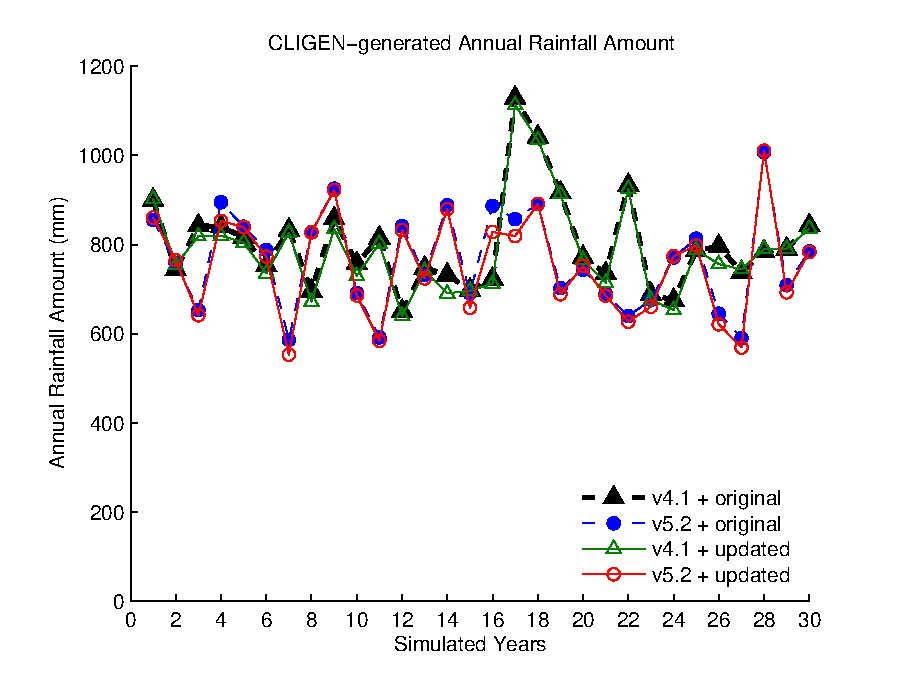
\includegraphics[width=0.8\textwidth]{./img/cligen_annual_amount_series}
  \caption{Simulated annual rainfall amount using two versions of CLIGEN
with original and updated input files.}
  \label{fig:cligen_annual_amount}
\end{figure}

\subsection{Rainfall Duration}
Contrastingly, simulated annual rainfall durations using two versions of CLIGEN
exhibited noticeable differences. Old version of CLIGEN generated identical
annual rainfall durations even though two different input files (original
and updated) were used (Figure \ref{fig:cligen_annual_duration}). New CLIGEN
generated markedly different rainfall durations when the same set of CLIGEN
input files were used (Figure \ref{fig:cligen_annual_duration}) (K-S test,
$p<0.05$).

\begin{figure}[htbp]
  \centering
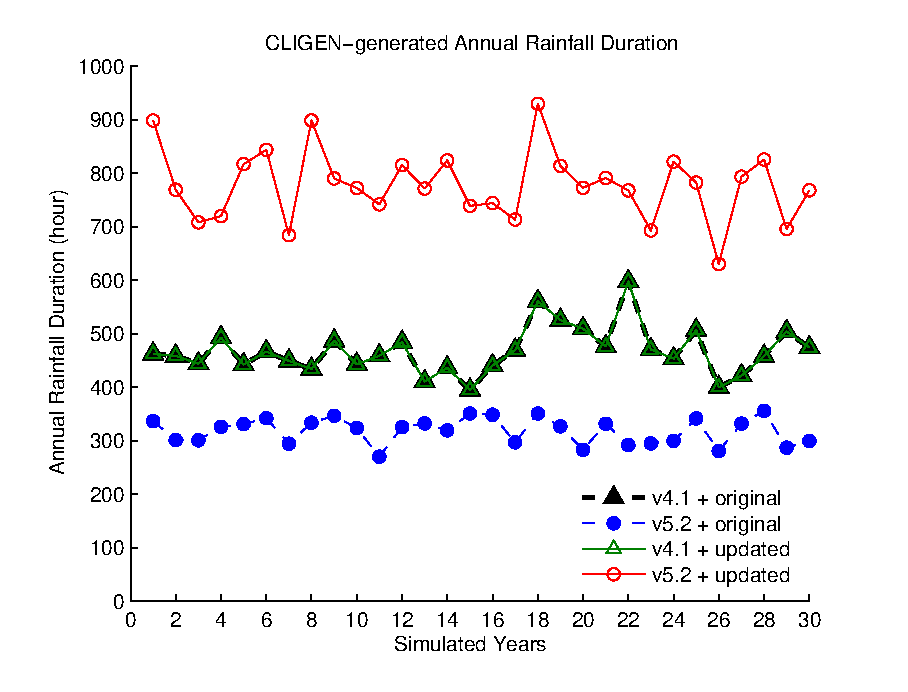
\includegraphics[width=0.8\textwidth]{./img/cligen_annual_duration_series}
  \caption{Simulated annual rainfall duration using two versions of CLIGEN
with original and updated input files.}
  \label{fig:cligen_annual_duration}
\end{figure}

New CLIGEN with updated input file generated greatly increased rainfall
durations, almost 2.5 times longer on average than with original input file. The
rainfall duration was over 1.5 times longer on average in comparison to the
rainfall duration generated by old CLIGEN. New CLIGEN with original input file
generated the shortest annual rainfall durations among the four series.
This means that, unlike old version, new version of CLIGEN is sensitive to
the change of two CLIGEN input parameters (i.e.\ MEAN~P and {MX.5P}),
particularly to the change of {MX.5P}. Great differences in rainfall durations
mean that rainfall intensities also differ greatly between the simulated
rainfall data.



\subsection{Monthly Maxima of Daily Peak Rainfall Intensity}
Next, monthly maxima of daily peak rainfall intensity series generated by CLIGEN
were compared in order to examine effects of extreme intensity events. The
results are shown in Figure \ref{fig:cligen_monthly_max_int}.
Kolmogorov-Smirnov tests indicate that old CLIGEN was not sensitive to the
changes of input files (See Figure \ref{fig:cligen_monthly_max_int}(a) and
\ref{fig:cligen_monthly_max_int}(c)) (i.e.\ to the changes of MEAN~P and
{MX.5P}) ($p<0.05$). In contrast, using original and updated input files with
new CLIGEN resulted in two significantly (K-S test, $p<0.05$) different
distributions of monthly maxima of daily peak rainfall intensity (See Figure
\ref{fig:cligen_monthly_max_int}(b) and \ref{fig:cligen_monthly_max_int}(d)).
New CLIGEN generated fewer high-peaked rainfall intensity events than the old
version (Figure \ref{fig:cligen_monthly_max_int}(a)(c) and
\ref{fig:cligen_monthly_max_int}(b)(d)). There were, for example, only nine
monthly maxima of daily peak intensity over 100 mm/hr during 30 years of the
simulation period when new CLIGEN and updated input file were used (Figure
\ref{fig:cligen_monthly_max_int}(d)). The magnitude of the monthly maxima of the
daily peak intensity seems to be in a similar range for all four cases although
the frequency of such high values may vary depending on versions of CLIGEN and
input files.

\begin{figure}[htbp]
  \centering

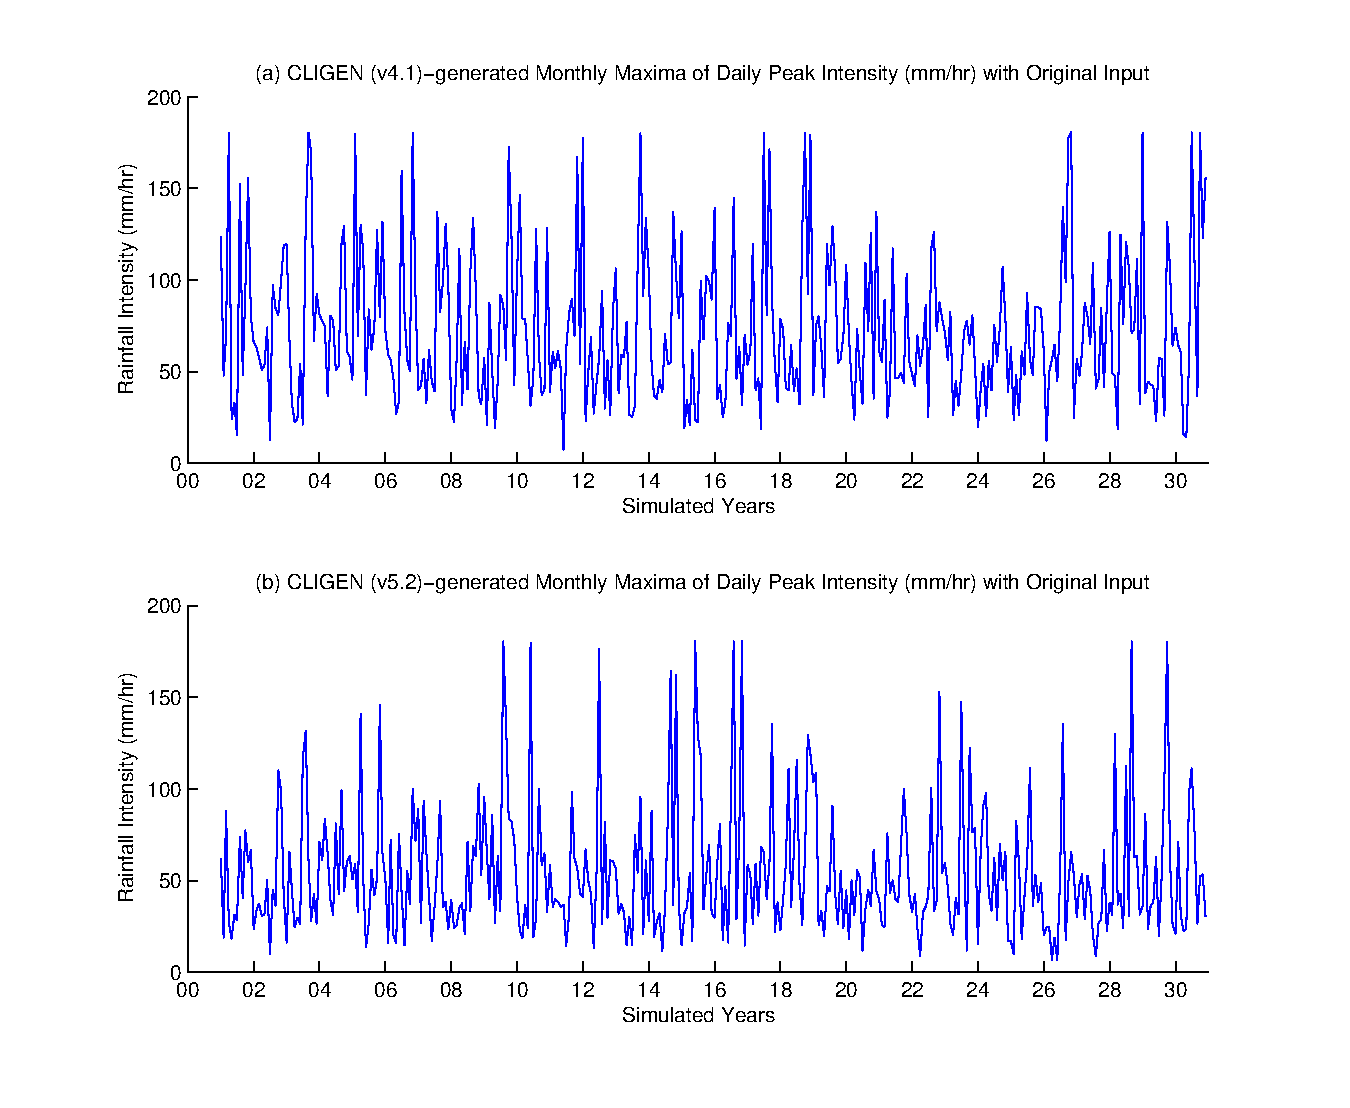
\includegraphics[width=0.8\textwidth]{./img/cligen_monthly_max_int_org}

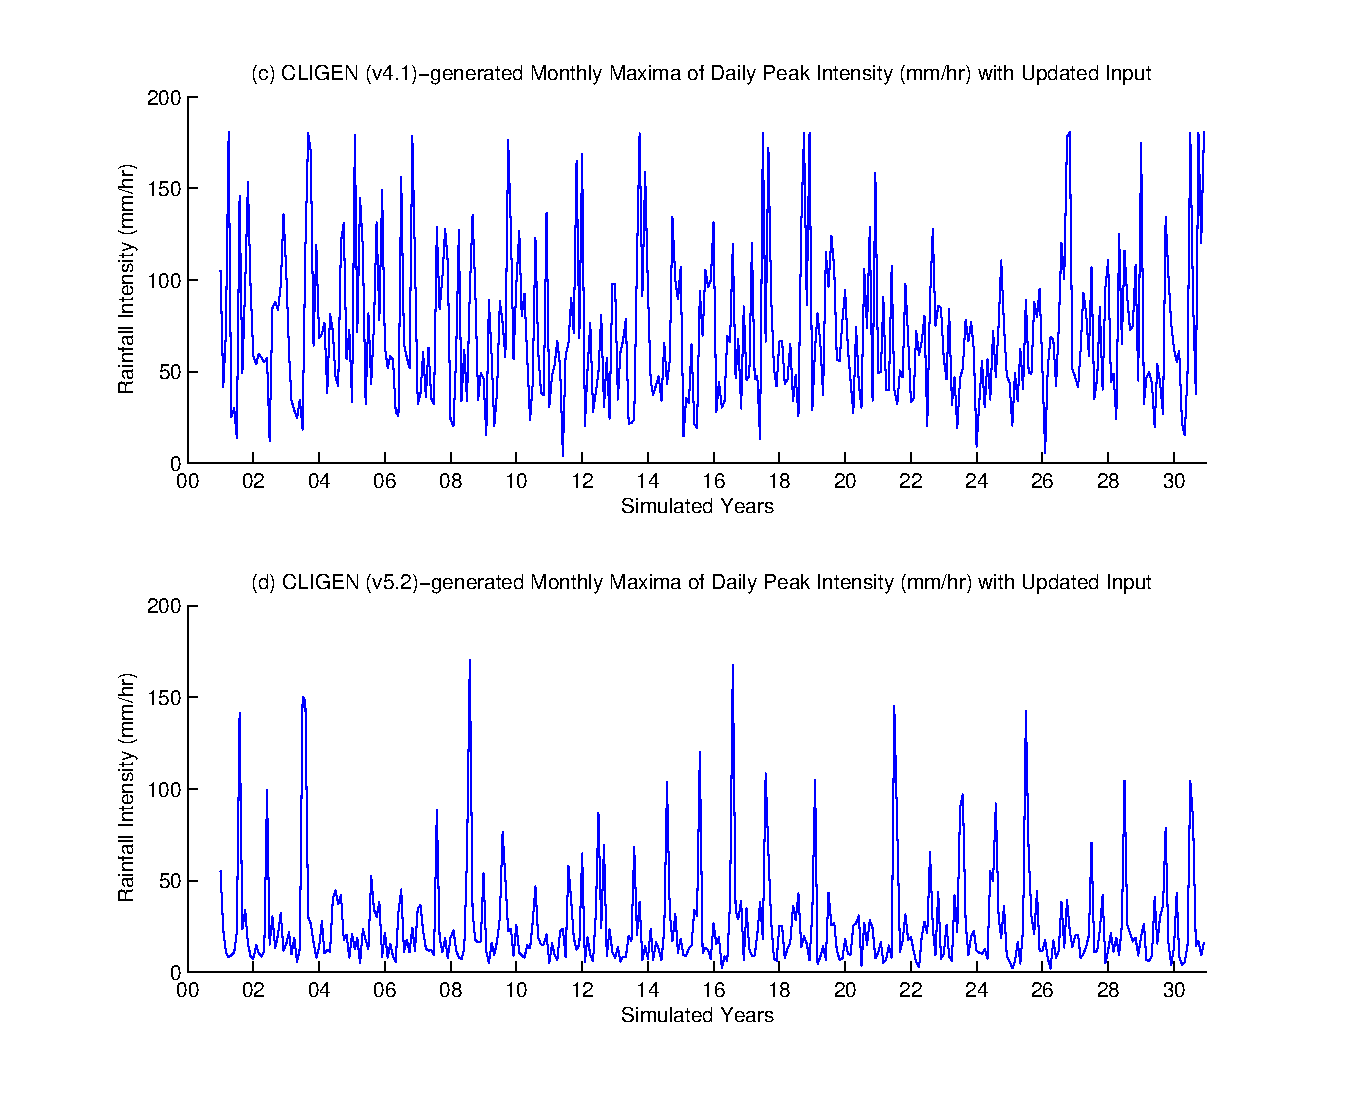
\includegraphics[width=0.8\textwidth]{./img/cligen_monthly_max_int_mod}
  \caption[Simulated monthly maxima of daily peak rainfall intensity using
two versions of CLIGEN with original and updated input files]{Simulated monthly
maxima of daily peak rainfall intensity using two versions of CLIGEN with
original and updated input files. (a) CLIGEN v4.1 with original input file; (b)
CLIGEN v5.2 with original input file; (c) CLIGEN v4.1 with updated input file;
(d) CLIGEN v5.2 with updated input file.}
  \label{fig:cligen_monthly_max_int}
\end{figure}

\begin{figure}[htbp]
  \centering

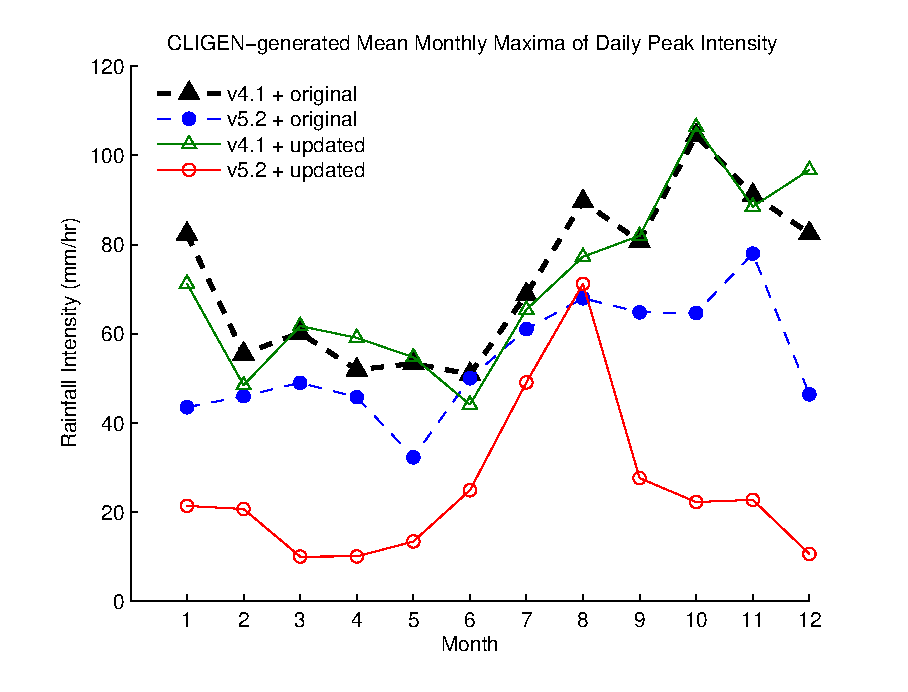
\includegraphics[width=0.8\textwidth]{./img/cligen_monthly_max_int_by_month}
  \caption{CLIGEN-generated mean monthly maxima of daily peak intensity
using two versions of CLIGEN with original and updated input files}
  \label{fig:cligen_dr_monthly_max_int_by_month}
\end{figure}

Mean monthly maxima of daily peak intensity were compared in Figure
\ref{fig:cligen_dr_monthly_max_int_by_month}. Old CLIGEN with two input files
generated generally high mean monthly values through out all months in
comparison to new CLIGEN. The effect of different input files was very small
with old CLIGEN on simulated mean monthly maxima of daily peak intensity. Old
CLIGEN generated highest mean monthly maxima of daily peak intensity in October
and lowest values in June with both input files. In contrast, new CLIGEN
generated significantly different mean monthly maxima of daily peak intensity
with two input files (K-S test, $p<0.05$). Much greater mean monthly maxima of
daily peak intensity were generated with original input file and new CLIGEN than
with updated input file. With original input file, new CLIGEN showed a peak in
November and a low in May.

With exception of new CLIGEN with the updated input file, all three simulations
show generally high mean monthly maxima of daily peak intensity in October and
November and low mean monthly maxima of daily peak intensity in April, May and
June. When new CLIGEN with updated input file were used for the simulation, the
monthly pattern was very different from that of the other three combinations.
This combination (new CLIGEN with updated input file) showed relatively high
mean monthly maxima of daily peak intensity during the summer months (June, July
and August) with a distinctively high peak in August (Figure
\ref{fig:cligen_dr_monthly_max_int_by_month}). Generally low mean monthly maxima
of daily peak intensity in the rest of months were simulated with lowest mean
monthly maxima of daily peak intensity in March and April (Figure
\ref{fig:cligen_dr_monthly_max_int_by_month}). With updated input file and new
CLIGEN, more high intensity events were simulated in the summer than the autumn
or winter in comparison to the other simulation combinations.
%reason for this result can be explained by looking at the input files, october
%and august, MEAN P and MX .5P

\section{Implication on Runoff and Soil Erosion Simulation}
\label{sec:RunoffAndSoilLossSimulation}
Before starting investigations on effects of improved CLIGEN on WEPP
simulations, initial tests of WEPP were carried out with weather generated by
new CLIGEN with updated input file. The tests revealed that uncalibrated WEPP
overestimates mean soil loss by about 630\% in comparison to observed soil
losses from the study area (Table
\ref{tab:SimulatedSoilLossWithCLIGENV52WithUpdatedInput}). This erosion rate is
considered undesirably high for the study site so that calibrations is
deemed to be essential. Thus, WEPP was calibrated by adjusting hydrological and
erosional parameter values. The adjusted parameters were shown in Table
\ref{tab:HydrologicalAndErosionalParameters}. Simulated runoff and soil loss
rates using uncalibrated and calibrated WEPP are presented in Table
\ref{tab:SimulatedRunoffWithCLIGENV52WithUpdatedInput} and
\ref{tab:SimulatedSoilLossWithCLIGENV52WithUpdatedInput}. No measured runoff
data were available for the site.

\begin{table}[htbp]
  \figureversion{tabular}
  \centering
  \caption[Simulated annual average runoff on hillslopes using
CLIGEN-generated weather with updated input]{Simulated annual average runoff
(mm) on hillslopes (D-L) using CLIGEN-generated (v5.2) weather with updated
input}
  \label{tab:SimulatedRunoffWithCLIGENV52WithUpdatedInput}
  \small
    \begin{tabular}{lrrrrrrrrrr}
      \toprule
      & D & E & F & G & H & I & J & K & L & Mean\\
      \cmidrule{2-11}
      uncalib. & 106.7 & 105.3 & 106.5 & 106.0 & 106.1 & 107.1
& 107.8 & 108.0 & 108.8 & 106.9\\
      recalib. & 74.2 & 72.9 & 73.9 & 73.6 & 73.4 & 74.3 &
74.8 & 75.2 & 75.9 & 74.2\\
      \bottomrule
    \end{tabular}
\end{table}

\begin{table}[htbp]
  \figureversion{tabular}
  \centering
  \caption[Simulated annual average soil loss on hillslopes using
CLIGEN-generated weather with updated input]{Simulated annual average soil loss
(t/ha) on hillslopes (D-L) using CLIGEN-generated (v5.2) weather with updated
input}
  \label{tab:SimulatedSoilLossWithCLIGENV52WithUpdatedInput}
  \footnotesize
    \begin{tabular}{lrrrrrrrrrr}
      \toprule
      & D & E & F & G & H & I & J & K & L & Mean\\
      \cmidrule{2-11}
      uncalibrated & 49.4 & 42.9 & 76.1 & 96.5 & 117.5 & 111.1
& 105.3 & 84.1 & 79.7 & 84.7\\
      recalibrated & 3.4 & 3.2 & 11.1 & 18.2 & 23.7 & 21.3 &
17.3 & 9.8 & 7.9 & 12.8\\
      measured$^a$ (m$^3$/ha) & 3.4 & 7.8 & 13.7 & 17.5 & 21.4
& 9.6 & 11.6 & 11.2 & 8.1 & 11.6\\
      \bottomrule
      %\addlinespace[1mm]
      \multicolumn{8}{l}{\footnotesize $^a$ over the periods
of 1985-1986 \citep[From][]{favis-mortlock1998-141}}
    \end{tabular}
\end{table}

Using only relative representations (\% change) of model outputs might seem more
meaningful than using absolute values (t/ha) together with \% changes in this
research because what this research is interested in is how model estimates
change as a result of rainfall-intensity changes. However, in order to make
right judgement and to assess the estimated values correctly, we need both
expressions: \% change and absolute value. For instance, if a model estimates
soil loss of 1000 t/ha from a 1 m $\times$ 1 m plot after 10 mm/hr rainfall, it
would hardly be considered realistic, and the model and its inputs may need to
be checked for any error. On the other hand, when a model estimates soil loss
that changes from, say, 0.00001 t/ha to 0.00002 t/ha, the \% change would be
100\% despite the fact that this value can be seen as very trivial in the real
world. Thus, presenting the model result either only in \% change or absolute
value could lead to a wrong conclusion. Therefore, both expressions are used in
this research when simulation results are presented.

Moreover, it is paramount to test and calibrate a model before using it in the
subsequent investigation of this research. With model calibrations, high
correlations can be expected \citep{jetten1999-521,favis-mortlock1998-141}. When
a erosion model is used for soil loss estimations, it is important to note that
the relationship of model inputs and outputs is non-linear. For example, say, we
ran a erosion model with $Input A$ and got $Output B$. Then, in order to find
possible effects of changes in inputs, we may change $Input A$ to $Input A'$.
When the model was run with $Input A'$, the responding model output should be
$Output B'$ if the model has a linear relationship between inputs and outputs.
However, because of the non-linear relationship, the responding output may be
rather unknown $Output B''$. This means that, unless model inputs and
outputs are identified and the model is calibrated against known output values,
it may be difficult to measure the extent of changes in model predictions. This
is because we may not know where unknown $Output B''$ has arrived from.

WEPP simulated annual runoff and soil loss rates using four CLIGEN-generated
weather series are shown in Figure \ref{fig:cligen_annual_runoff_serise} and
Figure \ref{fig:cligen_annual_sloss_series}, respectively.

\begin{figure}[htbp]
  \centering
    \subfloat[]{%
    \label{fig:cligen_annual_runoff_serise_a}
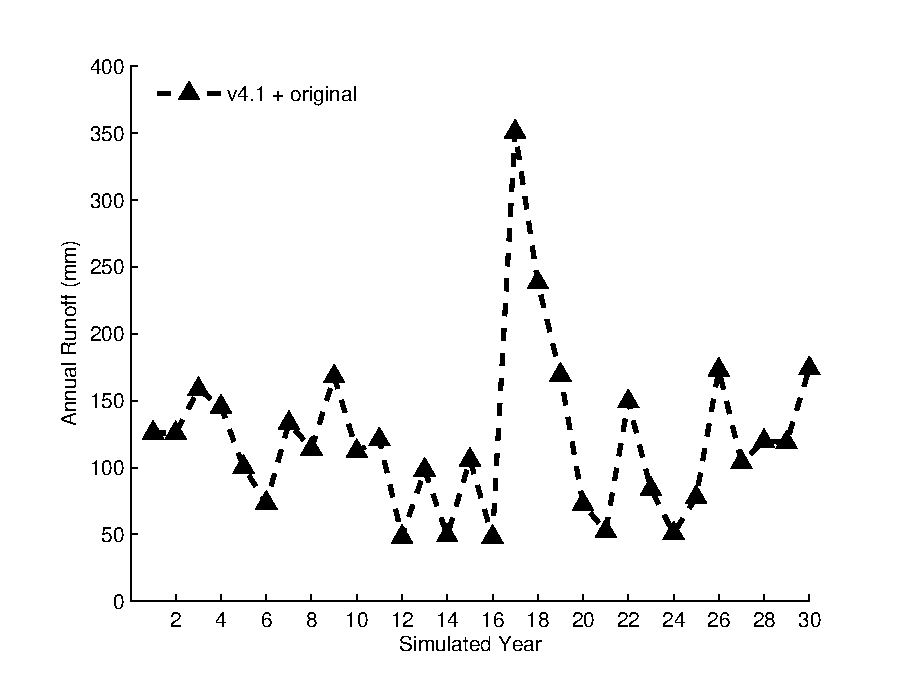
\includegraphics[width=0.49\textwidth]
{./img/cligen_annual_runoff_serise_old_original}}
    \subfloat[]{%
    \label{fig:cligen_annual_runoff_serise_b}
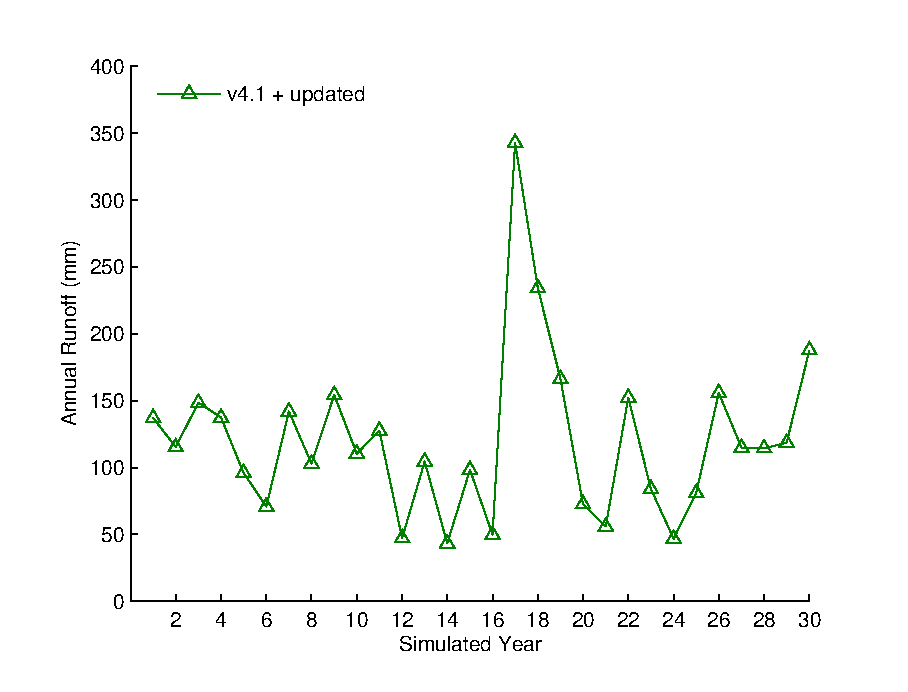
\includegraphics[width=0.49\textwidth]{%
./img/cligen_annual_runoff_serise_old_updated}}
    \qquad
    \subfloat[]{%
    \label{fig:cligen_annual_runoff_serise_c}
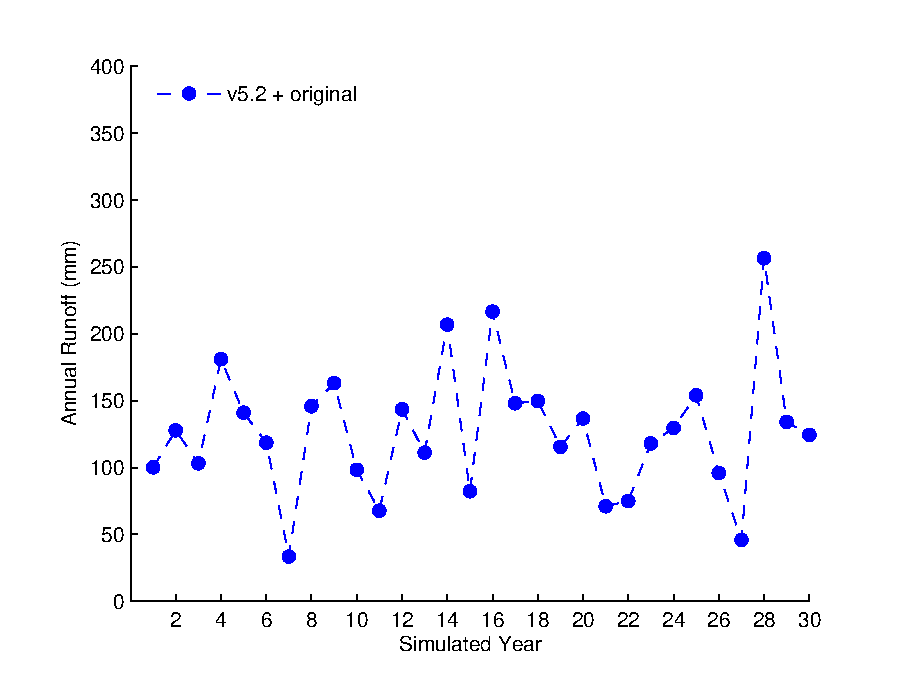
\includegraphics[width=0.49\textwidth]{%
./img/cligen_annual_runoff_serise_new_original}}
    \subfloat[]{%
    \label{fig:cligen_annual_runoff_serise_d}
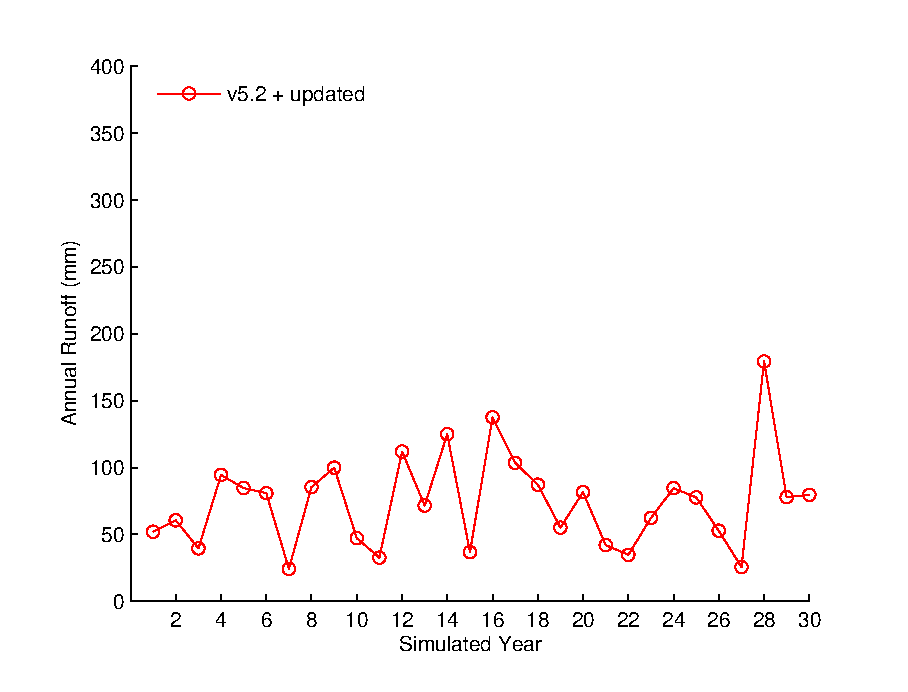
\includegraphics[width=0.49\textwidth]{%
./img/cligen_annual_runoff_serise_new_updated}}
  \caption[Simulated annual runoff for Ditchling Road]{Simulated annual
runoff for Ditchling Road simulated with (a) old CLIGEN with original input
file; (b) old CLIGEN with updated input file; (c) new CLIGEN with original input
file; (d) new CLIGEN with updated input file.}
  \label{fig:cligen_annual_runoff_serise}
\end{figure}

\begin{figure}[htbp]
  \centering
  \subfloat[]{%
  \label{fig:cligen_annual_sloss_series_a}
  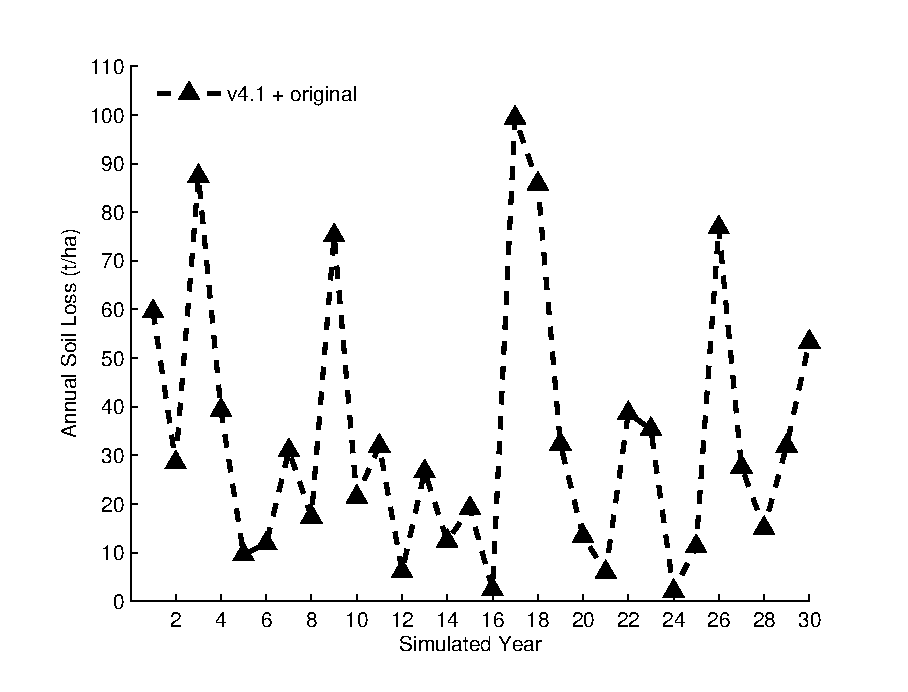
\includegraphics[width=0.49\textwidth]{%
./img/cligen_annual_sloss_serise_old_original}}
  \subfloat[]{%
  \label{fig:cligen_annual_sloss_series_b}
  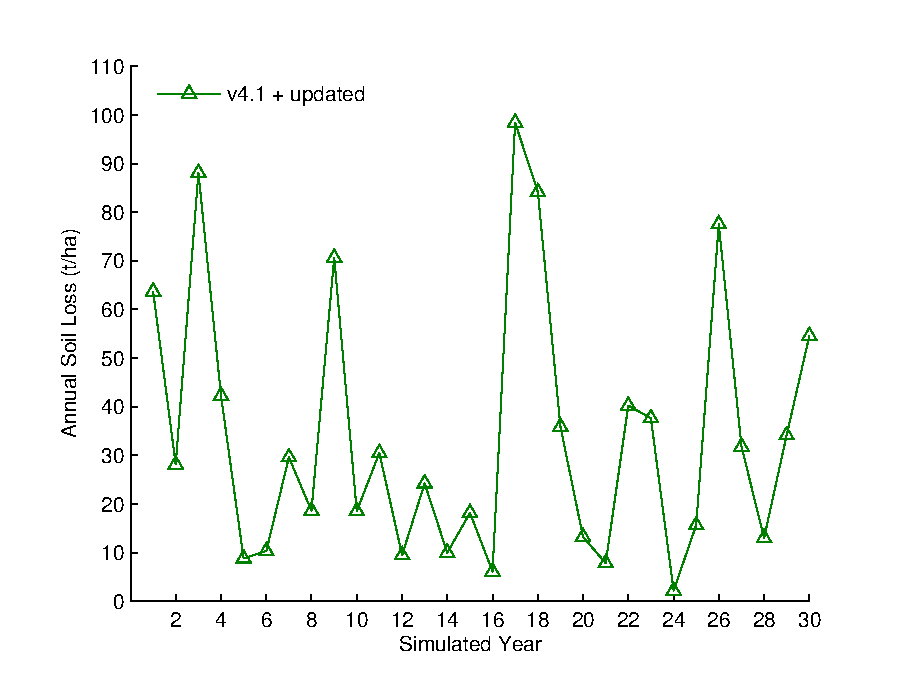
\includegraphics[width=0.49\textwidth]{%
./img/cligen_annual_sloss_serise_old_updated}}
  \qquad
  \subfloat[]{%
  \label{fig:cligen_annual_sloss_series_c}
  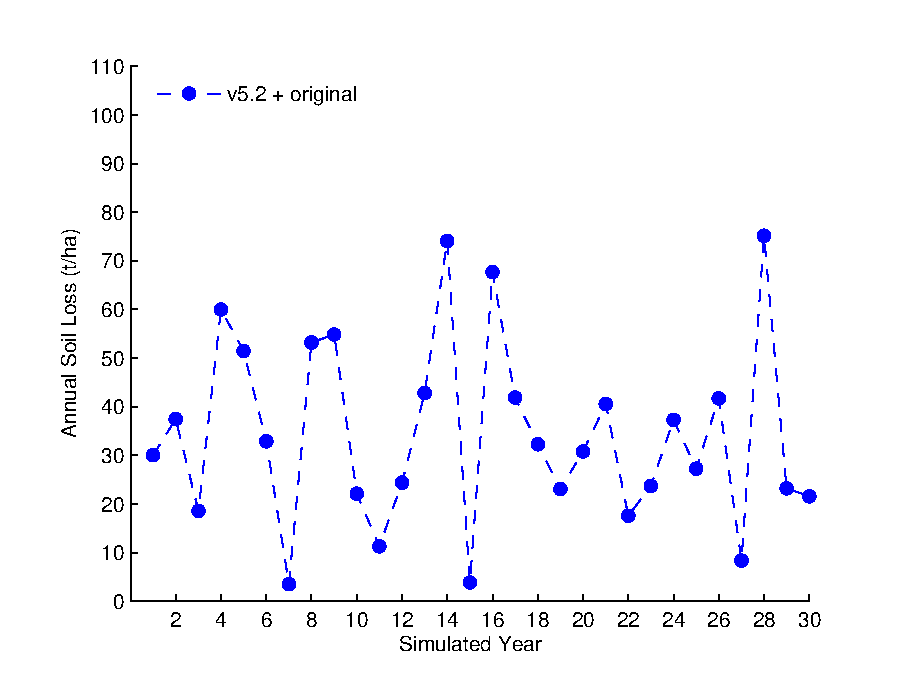
\includegraphics[width=0.49\textwidth]{%
./img/cligen_annual_sloss_serise_new_original}}
  \subfloat[]{%
  \label{fig:cligen_annual_sloss_series_d}
  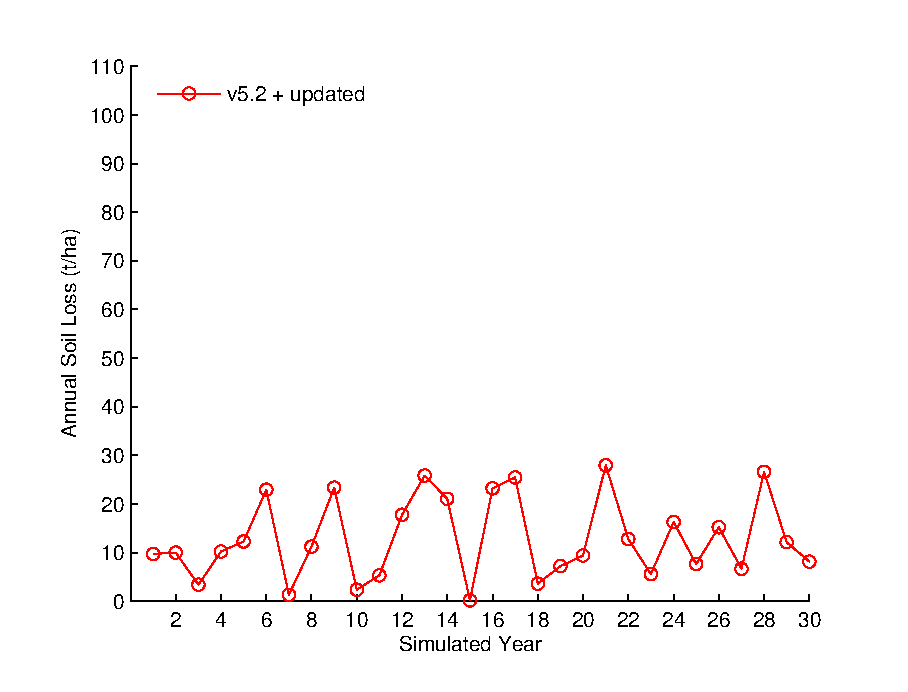
\includegraphics[width=0.49\textwidth]{%
./img/cligen_annual_sloss_serise_new_updated}}
  \caption[Simulated annual soil loss for Ditchling Road]{Simulated annual
soil loss for Ditchling Road simulated with (a) old CLIGEN with original input
file; (b) old CLIGEN with updated input file; (c) new CLIGEN with original input
file; (d) new CLIGEN with updated input file.}
  \label{fig:cligen_annual_sloss_series}
\end{figure}

Annual runoff and soil loss rates were not significantly affected by the use of
climate datasets that have been generated by two input files with old CLIGEN.
Annual runoff (Figure \ref{fig:cligen_annual_runoff_serise_a} and Figure
\ref{fig:cligen_annual_runoff_serise_b}) and annual soil loss rates (Figure
\ref{fig:cligen_annual_sloss_series_a} and Figure
\ref{fig:cligen_annual_sloss_series_b}) were almost identical between the two
configurations (old CLIGEN with original and updated input files). Mean annual
runoff and soil loss rates estimated using climate data generated by old CLIGEN
with updated input file were slightly decreased 1.4\% and increased 1.5\%
respectively in comparison to the estimation by the use of old CLIGEN with
original input file (Table
\ref{tab:SimualtedAnnualRunoffAndSoilLossWithDifferentConfiguration}).

\begin{table}[htbp]
  \figureversion{tabular}
  \centering
  \caption[WEPP simulated average annual runoff and soil loss]{WEPP
simulated average annual runoff (mm) and soil loss (t/ha) with CLIGEN generated
weather with four different configurations.}
  \label{tab:SimualtedAnnualRunoffAndSoilLossWithDifferentConfiguration}
    \begin{tabular}{lrrrr}
      \toprule
       & \multicolumn{2}{c}{CLIGEN v4.1} &
\multicolumn{2}{c}{CLIGEN v5.2}\\
      \cmidrule(r){2-3}\cmidrule(l){4-5}
       & original input & updated input & original input &
updated input \\
      \midrule
      Runoff & 122.1 & 120.4 ($-$1.4) & 126.5 ($+$3.6) & 74.2
($-$39.2)\\
      Soil Loss & 33.6 & 34.1 ($+$1.5) & 34.4 ($+$2.4) & 12.8
($-$61.9)\\
      \bottomrule
      %\addlinespace[1mm]
      \multicolumn{5}{p{10.5cm}}{\footnotesize Figures in (\ )
represent \% differences from CLIGEN v4.1+original input file. $+/-$ sign
indicates an increase/decrease.}
    \end{tabular}
\end{table}

WEPP with climate data generated by new CLIGEN with original input file
estimated the similar average annual runoff and soil loss rates from those
simulated with old CLIGEN with original input file with 3.6\% and 2.4\%
increases, respectively (Table
\ref{tab:SimualtedAnnualRunoffAndSoilLossWithDifferentConfiguration}). However,
annual runoff and soil loss rates estimated by the use of climate data generated
with new CLIGEN were significantly different from annual runoff and soil loss
rates estimated using climate data from old CLIGEN (Figure
\ref{fig:cligen_annual_runoff_serise} and \ref{fig:cligen_annual_sloss_series}).

WEPP estimated considerably decreased runoff and soil loss rates when climate
data from new CLIGEN with updated input file were used in comparison to the
other three configurations (Figure \ref{fig:cligen_annual_runoff_serise_d} and
Figure \ref{fig:cligen_annual_sloss_series_d}). In comparison to mean runoff and
soil loss rates estimated by the use of old CLIGEN with original input file,
mean annual runoff and soil loss rates decreased about 40\% and about 62\%
respectively when climate data from new CLIGEN with updated input file were used
for WEPP simulations (Table
\ref{tab:SimualtedAnnualRunoffAndSoilLossWithDifferentConfiguration}).

\section{Discussion}
\label{sec:ImprovedCLIGENDiscussion}

\subsection{Impact on Rainfall Data Generation}

\citet{yu2000-301} suggests that CLIGEN became sensitive to the changes in
rainfall intensity parameters after the corrections. The investigation conducted
here confirms this improvement. Rainfall duration generated by new CLIGEN (v5.2)
showed a clear evidence of this improvement (Figure
\ref{fig:cligen_annual_duration}).

Updated CLIGEN input file that includes lower {MX.5P} values than original input
file resulted in longer rainfall durations as shown in Figure
\ref{fig:cligen_annual_duration}. This was expected because of the lower {MX.5P}
values and the similar MEAN~P values in updated input file (Figure
\ref{fig:mean_p_mx5p_cligen}). With rainfall amount almost unchanged---only
slightly changed, but statistically the same ($p<0.05$), rainfall duration has
to be increased to satisfy low intensity parameter (Figure
\ref{fig:cligen_annual_duration}). This, in turn, decreases generated rainfall
intensity (Figure \ref{fig:cligen_dr_monthly_max_int_by_month}).

Old CLIGEN did not show much changes in rainfall intensity even though the
rainfall intensity parameters ({MX.5P}) were updated to the lower values when
preparing original and updated input files. This insensitivity of old CLIGEN is
clearly the result of the unit conversion error previously found by
\citet{yu2000-301}. Correcting the errors in the previous version of CLIGEN
resulted in decreased rainfall intensity (Figure
\ref{fig:cligen_dr_monthly_max_int_by_month}).

New CLIGEN with the updated input file simulated a peak monthly intensity in
August that can also be seen in input file (Figure
\ref{fig:cligen_dr_monthly_max_int_by_month} and Figure \ref{fig:mx5p_cligen}).
This means that new CLIGEN generates monthly rainfall intensity that are similar
to {MX.5P} values which are calculated from observed weather data.

Old CLIGEN generated the similar monthly rainfall intensity for both input
files. This implies that old CLIGEN does not recognize the intensity differences
introduced by the different {MX.5P} parameters in the original input file.

\begin{figure}[htbp]
  \centering
    \subfloat[MEAN P]{\label{fig:mean_p_cligen}
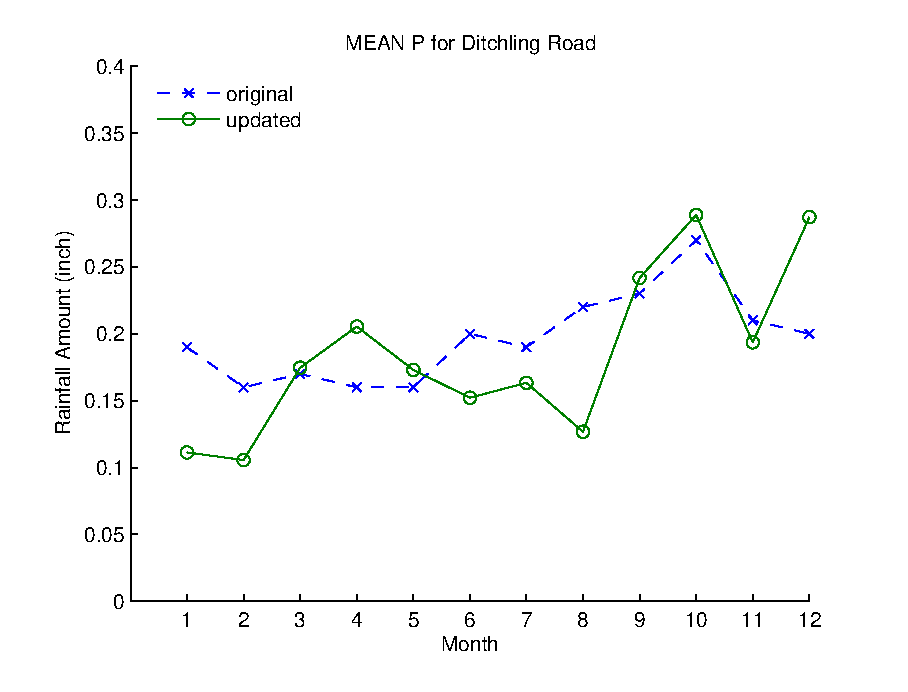
\includegraphics[width=0.49\textwidth]{./img/mean_p_cligen}}
    \subfloat[MX .5P]{\label{fig:mx5p_cligen}
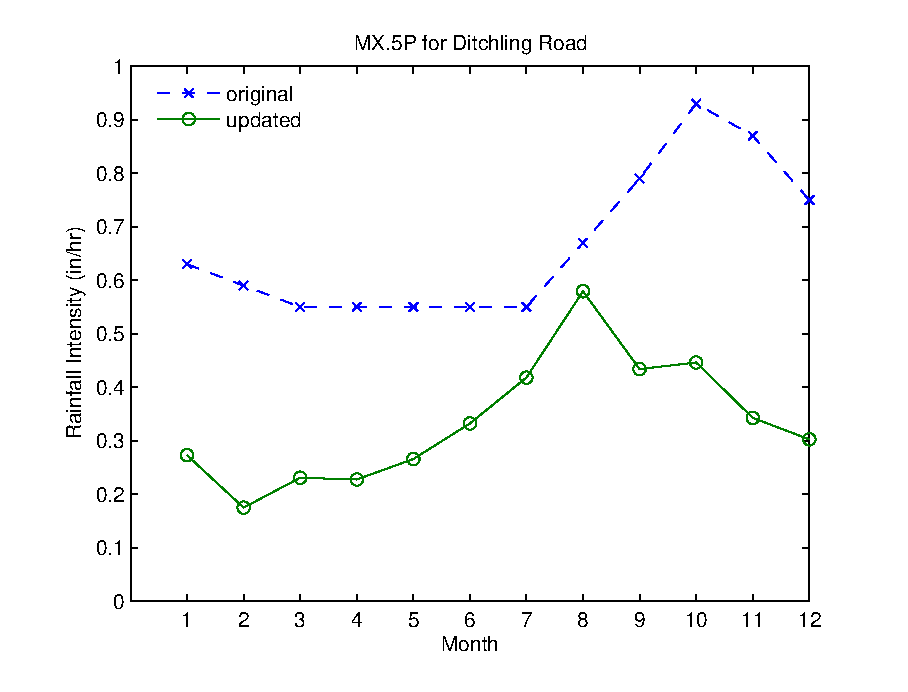
\includegraphics[width=0.49\textwidth]{./img/mx5p_cligen}}
  \caption[Mean daily precipitation depth and mean maximum daily 30-minute
rainfall intensity for each month]{Mean daily precipitation depth (inch) and
mean maximum daily 30-minute rainfall intensity (in/hr) for each month. Note
that the units are in inches, not in millimetres, as CLIGEN requires these
values in inches.}
  \label{fig:mean_p_mx5p_cligen}
\end{figure}

\subsection{Impact on Runoff and Soil Loss Estimation}

Runoff and soil erosion estimated by WEPP showed the similar result to that from
the analysis of climate data generated by CLIGEN. This result may imply that
WEPP is sensitive to the changes of climate data which have been used for the
simulation.

The two identical climate datasets generated by old CLIGEN with two input files
did not affect WEPP estimated annual runoff (Figures
\ref{fig:cligen_annual_runoff_serise_a} and
\ref{fig:cligen_annual_runoff_serise_b}) and soil erosion rates (Figures
\ref{fig:cligen_annual_sloss_series_a} and
\ref{fig:cligen_annual_sloss_series_b}).
There were slight differences between two settings in terms of average annual
runoff and soil loss rates (Table
\ref{tab:SimualtedAnnualRunoffAndSoilLossWithDifferentConfiguration}). The
differences were however unrealistic as average annual soil loss rate was
increased even though average annual runoff was decreased. This suggests that
WEPP may have some issues in processing runoff and soil loss rate.

The use of two climate date from the new CLIGEN simulations with two input files
resulted in significantly different runoff and soil loss rates between two
settings of WEPP simulations. WEPP simulated considerably lower annual runoff
and soil loss rates when climate data generated by new CLIGEN with updated input
file were used than when climate data generated by new CLIGEN with original
input file were used. This can be explained by the stretched rainfall duration
which have been caused by the decreases in rainfall intensity. Considering that
simulated rainfall amounts (MEAN P) were not much different in both input files
of CLIGEN, it is evident that low rainfall intensity ({MX.5P}) is the reason for
the low annual runoff and annual soil loss rates estimated by WEPP.

Another interesting finding is that the differences of average annual runoff and
soil loss rates between the simulations of WEPP with new CLIGEN and old CLIGEN
with original input file were much smaller than with updated input file. This
finding may be explained by the differences in two versions of CLIGEN. New
CLIGEN, as shown earlier, is much more sensitive to changes in rainfall
intensity than old CLIGEN, so that, with CLIGEN input file that has low rainfall
intensity, new CLIGEN will simulate climate data with much lower rainfall
intensity. In contrast, with CLIGEN input file that has high rainfall intensity,
new CLIGEN still simulate climate data with responding rainfall intensity, that
is high rainfall intensity. This is clearly shown in Figure
\ref{fig:cligen_dr_monthly_max_int_by_month}.

Therefore, the implication of the improvement in CLIGEN is relatively small when
new CLIGEN is used to simulate climate data for a place where rainfall events
with high intensity are dominant. On the other hand, when new CLIGEN is used to
generate climate date for a place where rainfall events with low intensity are
dominant (e.g. South Downs, UK), effects on simulated climate data are so great
that following WEPP estimations will be greatly affected and have much greater
implications.


\section{Conclusion}
\label{sec:ImprovedCLIGENConclusion}
The improvement of CLIGEN have clear implications on climate data generations
and following WEPP estimations of runoff and soil loss rates. Old CLIGEN is not
sensitive to changes of rainfall intensity and generate the similar climate data
with both CLIGEN input files that have high and low intensity parameters. New
CLIGEN is now sensitive to changes in rainfall intensity which is parametrized
as {MX.5P}. The effect of the improvement of CLIGEN is more significant for the
regions where low intensity rainfall events are dominant. This is the case for
an area like South Downs, UK where this research is based on.


%\nolinenumbers

